%!TEX TS-program = xelatex
%!TEX encoding = UTF-8 Unicode

%% ZAKLADNI VLASTNOSTI STRANKY -- VELIKOST PISMA, STRANKY, OKRAJU
\documentclass[12pt,a4paper]{article}

%% XELATEX nastaveni fontu
%\usepackage{xltxtra,fontspec,xunicode}
%\setromanfont[Numbers=Uppercase]{Technika Light}
\usepackage{graphicx}
\usepackage[marginparsep=14pt,left=2.5cm,right=2.5cm,top=3.2cm,bottom=4.5cm]{geometry}

\usepackage{listings}
\lstset{
  basicstyle=\ttfamily,
  columns=fullflexible,
  breaklines=true,
  postbreak=\mbox{\textcolor{red}{$\hookrightarrow$}\space},
}

%% NASTAVENI MEZER
\setlength{\parskip}{8pt}
\setlength{\parindent}{25pt}

%% CESTINA
\usepackage[czech]{babel}
\usepackage[utf8]{inputenc}

%% VKLADANI ZDROJOVEHO KODU
%\usepackage{listings}

%% ZAHLAVI A ZAPATI
\usepackage{fancyhdr}
\pagestyle{fancy}
\renewcommand{\sectionmark}[1]{\markright{#1}}

% prostredni cast zapati
\cfoot{\thepage}

% leva cast zahlavi -- nazev sekce/subsekce
\lhead{\fancyplain{}{\rightmark}}

%\def\picturesfolder{images}
\graphicspath{ {./images/} }

% prava cast zahlavi -- logo fitu

\rhead{
\includegraphics[width=4cm]{logo}}

%% TABULKY
\usepackage{tabularx}

% podbarveni radku tabulek
\usepackage[table]{xcolor}

%% REJSTRIK -->
\usepackage{makeidx}
\makeindex
%% REJSTRIK <--

%% PROKLIKAVATELNE ODKAZY -- nastaveni xetex/pdftex
\usepackage[pdftex,pdfpagelabels,bookmarks,hyperindex,hyperfigures]{hyperref}

\hypersetup{
  colorlinks,
  citecolor=blue,
  filecolor=blue,
  linkcolor=blue,
  urlcolor=blue
}

% alternuj bilou a svetle sedou pro radky vsech tabulek
\rowcolors{1}{white}{gray!25}

\begin{document}
%%%%% TITLEPAGE

% bez cislovani stranek
\pagenumbering{gobble}

% bez cary oddelujici zahlavi a zapati
\renewcommand{\headrulewidth}{0pt}
\renewcommand{\footrulewidth}{0pt}

\begin{titlepage}
  % pro zobrazeni loga v zahlavi
  \thispagestyle{fancy}

  % vertikalni zarovnani
  \vspace*{\fill}
  \begin{center}
    {\fontsize{20}{30}\selectfont BI-BIG}\\[1cm]
    {\fontsize{30}{100}\selectfont \textbf{Semestrální práce}}\\[4.2cm]
  \end{center}

  % vertikalni zarovnani
  \vspace*{\fill}

  % seznam clenu tymu razeny abecedne podle krestniho jmena
  {\fontsize{10}{10} \selectfont \noindent
  \textbf{Autor:}\\
  Pavel Jahoda
  }
\end{titlepage}

\newpage

% cara nahore a dole oddelujici zahlavi a zapati od obsahu stranky
\renewcommand{\headrulewidth}{0.4pt}
\renewcommand{\footrulewidth}{0.4pt}


%%%%% OBSAH

% rimska cisla pro cislovani stranek v obsahu
\pagenumbering{roman}

% samotne vlozeni obsahu
\tableofcontents

\newpage

% zapnout bezne cislovani stranek pomoci arabskych cislic
\pagenumbering{arabic}

%%%%% TEXT

\section{Úvod}
Pro svoji záverečnou práci jsem se rozhodl použít reálná data charitativní organizace DonorsChoose.org, které podporuje veřejné vzdělání v USA. Data obsahují informace o dárcích, jednotlivé darované částky včetně dalších informacích o jednotlivých darech a v neposlední řadě obsahují stručné informace na co byli peníze využity. Nejprve jsem dělal agregace za použítí Spark, poté nahrál nástrojem Logstash\index{Logstash} data do vyhledávacího nástroje Elasticsearch\index{Elasticsearch}, kde jsem vytvořil index, který jsem využil na tvorbu grafů v Elasticsearch\index{Elasticsearch} pluginu Kibana\index{Kibana}.
%% REJSTRIK <--
%\index{ahoj}
%% REJSTRIK -->
\section{Data}
Data, která jsem využil naleznete na adrese \url{https://www.kaggle.com/donorschoose/io}. Z šesti možných csv souborů jsem si vybral, že budu pracovat s csv soubory Donations, Donors a Schools.
\subsection{Donors}
Donors obsahuje data o dárcích. Soubor \textit{Donors.csv} obsahuje okolo 2.1 milionů řádků. Data se skládají z 5 sloupců. Sloupec \textit{Donor ID} obsahuje hexadimální číslo, které reprezentuje identifikátor dárce. \textit{Donor City} a \textit{Donor State} obsahuje text reprezentující název města dárce a stát z kterého daný dárce pochází. Povolené znaky jsou a-z, A-Z nebo mezera. Sloupec \textit{Donor Is  Teacher} zodpovídá jestli je dárce učitel, povolené hodnoty jsou pouze "Yes" nebo "No". Poslední sloupec \textit{Donor Zip} obsahuje celá čísla 1-999 udávající první tři amerického ekvivalentu poštovního směrovacího čísla.
\begin{table}[!h]
\begin{tabularx}{1.05\textwidth}{lllXl}
Donor ID                         & Donor City   & Donor State & Donor Is Teacher & Donor Zip \\ \hline
00000ce845c00cbf0686c992fc369df4 & Evanston     & Illinois    & No               & 602       \\
00002783bc5d108510f3f9666c8b1edd & Appomattox   & other       & No               & 245       \\
00002d44003ed46b066607c5455a999a & Winton       & California  & Yes              & 953       \\
00002eb25d60a09c318efbd0797bffb5 & Indianapolis & Indiana     & No               & 462       \\
0000300773fe015f870914b42528541b & Paterson     & New Jersey  & No               & 75        \\
00004c31ce07c22148ee37acd0f814b9 &              & other       & No               &           \\
00004e32a448b4832e1b993500bf0731 & Stamford     & Connecticut & No               & 69        \\
00004fa20a986e60a40262ba53d7edf1 & Green Bay    & Wisconsin   & No               & 543       \\
00005454366b6b914f9a8290f18f4aed & Argyle       & New York    & No               & 128       \\
0000584b8cdaeaa6b3de82be509db839 & Valparaiso   & Indiana     & No               & 463      
\end{tabularx}
\caption{Donors}
\end{table}

\pagebreak
\subsection{Donations}
\flushleft{Donations obsahuje data o jednotlivých darech. Soubor \textit{Donations.csv} obsahuje okolo 4.7 milionů řádků. První tři sloupce zleva, neboli \textit{Project ID}, \textit{Donation ID} a \textit{Donor ID} obsahují unikátní identifikátory projektu, daru a dárce. Povolené hodnoty jsou pouze čísla v hexadecimální podobě. Sloupec \textit{Donation Included Optional Donation} obsahuje pouze hodnoty "No" a "Yes" a vyjadřuje jestli dárce dal 15\% z darované částky charitativní organizaci DonorsChoose. \textit{Donation Amount} je číslo vyjádřující darovanou částku. Darovaná částka může nabývat i desetinných hodnot. Sloupec \textit{Donor Cart Sequence} obsahuje celá čísla a poslední sloupec \textit{Donation Received Date} obsahuje datumy ve formátu "YYYY-MM-DD HH:MM:SS" a ukazují, kdy charita obdržela darovanou částku.}

\begin{table}[!htb]
\begin{tabularx}{1.1\textwidth}{XXXXXXX}
Project ID                       & Donation ID                      & Donor ID                         & Donation Included Optional Donation & Donation Amount & Donor Cart Sequence & Donation Received Date \\ \hline
000009891526c0ade7180f8423792063 & 688729120858666221208529ee3fc18e & 1f4b5b6e68445c6c4a0509b3aca93f38 & No                                  & 178.37          & 11                  & 2016-08-23 13:15:57    \\
000009891526c0ade7180f8423792063 & dcf1071da3aa3561f91ac689d1f73dee & 4aaab6d244bf3599682239ed5591af8a & Yes                                 & 25              & 2                   & 2016-06-06 20:05:23    \\
000009891526c0ade7180f8423792063 & 18a234b9d1e538c431761d521ea7799d & 0b0765dc9c759adc48a07688ba25e94e & Yes                                 & 20              & 3                   & 2016-06-06 14:08:46    \\
000009891526c0ade7180f8423792063 & 38d2744bf9138b0b57ed581c76c0e2da & 377944ad61f72d800b25ec1862aec363 & Yes                                 & 25              & 1                   & 2016-05-15 10:23:04    \\
000009891526c0ade7180f8423792063 & 5a032791e31167a70206bfb86fb60035 & 6d5b22d39e68c656071a842732c63a0c & Yes                                 & 25              & 2                   & 2016-05-17 01:23:38    \\
000009891526c0ade7180f8423792063 & 8cea27f0cc03f41f66aab96b284ae6a1 & 896c75c9b8d9a91c759746e566cd3f37 & Yes                                 & 15              & 1                   & 2016-06-04 17:58:55    \\
00000ce845c00cbf0686c992fc369df4 & 39af862cb04e4f938e5b827236a610a6 & 8a1875762c85932fff192ea126ccdff2 & Yes                                 & 50              & 1                   & 2013-02-27 09:07:51    \\
00000ce845c00cbf0686c992fc369df4 & c47f78571f62bcf10eee6a46a4a8a85d & a3f070e439d52de72ca62dc41f9b16a4 & Yes                                 & 50              & 2                   & 2013-02-27 09:53:12    \\
00000ce845c00cbf0686c992fc369df4 & 19351e1d9ae0bccab31b1f6009ad47a3 & bd323208dc78b1c74b62664b768f3176 & Yes                                 & 200             & 2                   & 2013-02-17 21:36:24    \\
00000ce845c00cbf0686c992fc369df4 & d5364b1bb3b14594808bd6efa7544165 & 6dd6113f89f2766d3b0707ef2a46260c & Yes                                 & 10              & 44                  & 2013-02-27 10:32:22   
\end{tabularx}
\caption{Donations}
\end{table}
\pagebreak
\subsection{Schools}
\flushleft{Schools obsahuje data o jednotlivých školách zapojených v projektu. Soubor \textit{Schools.csv} obsahuje okolo 70 tisíc řádků. Soubor má 6 sloupců z nichž první je unikátní identifikátor v podobě hexadecimálního čísla. Sloupec \textit{School Name} reprezentuje název školy. Přijatelné hodnoty jsou textové řetězce obsahující znaky a-z, A-Z nebo mezeru. \textit{School Metro Type} popisuje jakého je typu z hlediska urbanismu. Povolené hodnoty jsou "rural", "suburban", "urban" nebo "unknown". Sloupec \textit{School Percentage Free Lunch} udává procento žáků, kteří dostávají v rámci sociální podpory obědy zdarma. Povolené hodnoty jsou celá čísla od 0 do 100. Sloupec \textit{School State} obsahuje textový řetězec, který říká ve kterém státě se škola nachází a sloupec \textit{School Zip} obsahuje celá čísla 10000 až 99999 udávající americký ekvivalent poštovního směrovacího čísla.}

\begin{table}[htb]
\begin{tabularx}{1.05\textwidth}{XlXXXX}
School ID                        & School Name                            & School Metro Type & School Percentage Free Lunch & School State   & School Zip \\ \hline
00003e0fdd601b8ea0a6eb44057b9c5e & Capon Bridge Middle School             & rural             & 56                           & West Virginia  & 26711      \\
00004e32a448b4832e1b993500bf0731 & The Woodlands College Park High School & urban             & 41                           & Texas          & 77384      \\
0002021bb799f28de224f1acc1ff08c4 & Samantha Smith Elementary School       & suburban          & 2                            & Washington     & 98074      \\
0004604f675212a8cac1161338265196 & Kingsbury Country Day School           & unknown           & 76                           & Michigan       & 48370      \\
0004c9d50bcf0cea990f844e58b5e2c3 & Redwater Elementary School             & rural             & 50                           & Texas          & 75573      \\
0004ffe3558fd70d939ad522b92447c8 & Math \& Science Success Academy        & unknown           & 63                           & Arizona        & 85706      \\
000622b5ef4515b583da788f20be16ca & Harbor Science \& Arts Charter School  & urban             & 17                           & New York       & 10029      \\
000630ab66464a738cab5036738075df & Spears Creek Child Development Center  & unknown           & 15                           & South Carolina & 29045      \\
00064eac8b3d1f6dea8a07559922ed58 & Leadership Public School               & urban             & 46                           & California     & 95122      \\
0006658276977eeefb5bc7b0c7399b5b & Henking Primary School                 & suburban          & 29                           & Illinois       & 60025 
\end{tabularx}
\caption{School}
\end{table}

\section{Postup}
\subsection{Nahrání dat do Sparku\index{Spark}}
První úkol bylo vytvořit nový dataset, který bude agregovat data z jednoho původního datasetu. Tento bod, stejně jako další agregační úkoly jsem dělal ve Sparku\index{Spark}. Nejprve jsem všechny 3 csv soubory nahrál do sparku\index{Spark}. Postup byl následující.
\begin{lstlisting}
    cd BIG-FinalProject/spark
    docker build -f spark.df -t spark .
    docker-compose up -d
\end{lstlisting}

Data do sparku\index{Spark} nahrajeme z Hadoop distribuovaného file systému HDFS\index{HDFS}, takže neprve je do HDFS\index{HDFS} musíme dostat a to následujícími příkazy v nové příkazové řadce.
\begin{lstlisting}
    docker run --name hadoop -v /home/pjahoda/FIT/BIG/BIG-FinalProject/logstash/datasets/:/tmp/datasets -t -i sequenceiq/hadoop-docker /etc/bootstrap.sh -bash
    export PATH=$PATH:/usr/local/hadoop/bin/
    hdfs dfs -mkdir /test
    hdfs dfs -put ./tmp/datasets/Donors.csv /test/Donors.csv
    hdfs dfs -put ./tmp/datasets/Donations.csv /test/Donations.csv
    hdfs dfs -put ./tmp/datasets/Schools.csv /test/Schools.csv
\end{lstlisting}

Poté v původní příkazové řádce spustíme container, který reprezentuje driver program a následně v jeho příkazové řádce spustíme spark-shell připojený na master. V mém připadě byla adresa masteru 172.17.0.2.
\begin{lstlisting}
    docker run -it -p 8088:8088 -p 8042:8042 -p 4041:4040 --name driver -h driver spark:latest bash
    spark-shell --master spark://172.17.0.2:7077
\end{lstlisting}

Ve spark\index{Spark} shellu nahrajeme data do proměnných se kterými budeme dále pracovat.
\begin{lstlisting}
    val donors = spark.sqlContext.read.format("csv").option("header", "true").option("inferSchema", "true").load("hdfs://172.17.0.5:9000/test/Donors.csv")
    val donations = spark.sqlContext.read.format("csv").option("header", "true").option("inferSchema", "true").load("hdfs://172.17.0.5:9000/test/Donations.csv")
    val schools = spark.sqlContext.read.format("csv").option("header", "true").option("inferSchema", "true").load("hdfs://172.17.0.5:9000/test/Schools.csv")
\end{lstlisting}

\subsection{Agregace na jednom datasetu}
První úkol, agregovat data z jednoho původního datasetu, splníme následujícím příkazem.
\begin{lstlisting}
    val result = donors.groupBy("Donor City").count()
\end{lstlisting}

\subsection{Agregace na dvou datasetech}
Další úkol bylo vytvořit nový dataset, který bude agregovat data ze dvou původních datasetů najednou. Nejprve jsem udělal inner join nad dárcema a jejich darama.
\begin{lstlisting}
    val donor = donors.select(donors("Donor ID").as("id"),donors("Donor City"),donors("Donor State"),donors("Donor Is Teacher"),donors("Donor Zip"))
    val tmp = donor.join(donations,$"id" === $"Donor ID", "inner")
\end{lstlisting}

V proměnné tmp mám nyní uložený výsledek joinu, který použiju na agregaci. Momentálně jsou v tabulce řádky se stejným ID dárce, jelikož jeden dárce může mít několik darů. Já jsem chtěl vedět kolik každý dárce daroval dohromady, nikoliv jednotlivé dary, takže jsem tabulku agregoval dle potřeby následujícím příkazem.
\begin{lstlisting}
    val grouped = tmp.groupBy("id","Donor City","Donor State","Donor Is Teacher","Donor Zip").agg(sum("Donation Amount"))
\end{lstlisting}

S výsledkem budu dále pracovat ve vizualizačním nástroji Ksibana\index{Kibana}, tudíž si ho uložím na svůj hostovský PC. Toho dosáhnu nejprve přesunutím na HDFS\index{HDFS} a pak z HDFS\index{HDFS} do složky v dockerovského image která je namountovaná na složku v hostovském PC. Přesun do HDFS\index{HDFS} ze Sparku\index{Spark} se provádí následovně.
\begin{lstlisting}
    grouped.repartition(1).write.format("com.databricks.spark.csv").option("header", "true").save("hdfs://172.17.0.5:9000/test/DonorsDonations.csv")
\end{lstlisting}
\pagebreak

\subsection{Agregace předchozí agregace}
V příkazové řádce kde máme spustěný container s HDFS\index{HDFS} napíšeme následující příkaz.
\begin{lstlisting}
    hadoop fs -copyToLocal /test/DonorsDonations.csv /tmp/datasets/DonorsDonations
\end{lstlisting}

Posledním agregačním úkolem bylo vytvořit nový dataset, který bude agregovat data ze dvou datasetů najednou, z čehož jeden bude výsledkem předchozí agregace a uložit ho zpět do databáze/na file systém.
\begin{lstlisting}
    val donationByCity = grouped.groupBy("Donor City").agg(sum("sum(Donation Amount)"))
    val res = result.select(result("Donor City").as("city"),result("count"))
    val finalResult = res.join(donationByCity,$"city" === $"Donor City", "inner")
    val fResult = finalResult.select(finalResult("Donor City"),finalResult("count").as("Number of donors"),finalResult("sum(sum(Donation Amount))").as("Donation Amount"))
    fResult.repartition(1).write.format("com.databricks.spark.csv").option("header", "true").save("hdfs://172.17.0.5:9000/test/DonationsByCity.csv")
\end{lstlisting}

Opět v příkazové řádce s HDFS napíšeme nasledující kopírující příkaz
\begin{lstlisting}
    hadoop fs -copyToLocal /test/DonationsByCity.csv /tmp/datasets/DonationsByCity
\end{lstlisting}

Nakonec provedeme následující kontrolní příkaz, který výsledek uložené agregace nahraje zpět do Sparku\index{Spark}.
\begin{lstlisting}
    val temporary = spark.sqlContext.read.format("csv").option("header", "true").option("inferSchema", "true").load("hdfs://172.17.0.5:9000/test/DonationsByCity.csv")
\end{lstlisting}
\pagebreak

\subsection{Index v Elasticsearch\index{Elasticsearch}}
Pro tvorbu indexu v Elasticsearch\index{Elasticsearch} jsem si zvolil dataset DonorsDonations o jehož vytváření si můžete přečíst v podsekci "Agregace na dvou datasetech". Po vytvoření příslušných Logstashových\index{Logstash} konfiguračních souborů (především Logstash\index{Logstash} pipeline, která obsahuje který csv soubor a jakým způsobem nahrát a transformovat do ElasticSearch indexu) stačilo pouze spustit docker-compose.
\begin{lstlisting}
    cd BIG-FinalProject
    docker-compose up -d
\end{lstlisting}

\subsection{Vizualizace dat}
Na vizualizaci dat z datasetu DonorsDonations jsem použil nástroj Kibana\index{Kibana}. V Kibaně\index{Kibana} jsem si v sekci "Management" zvolil příslušný index a poté vytvořil několik vizualizací v sekci "Visualization". Na závěr jsem tyto vizualizace naskládal do jedné obrazovky v sekci "Dashboard".
\begin{center}
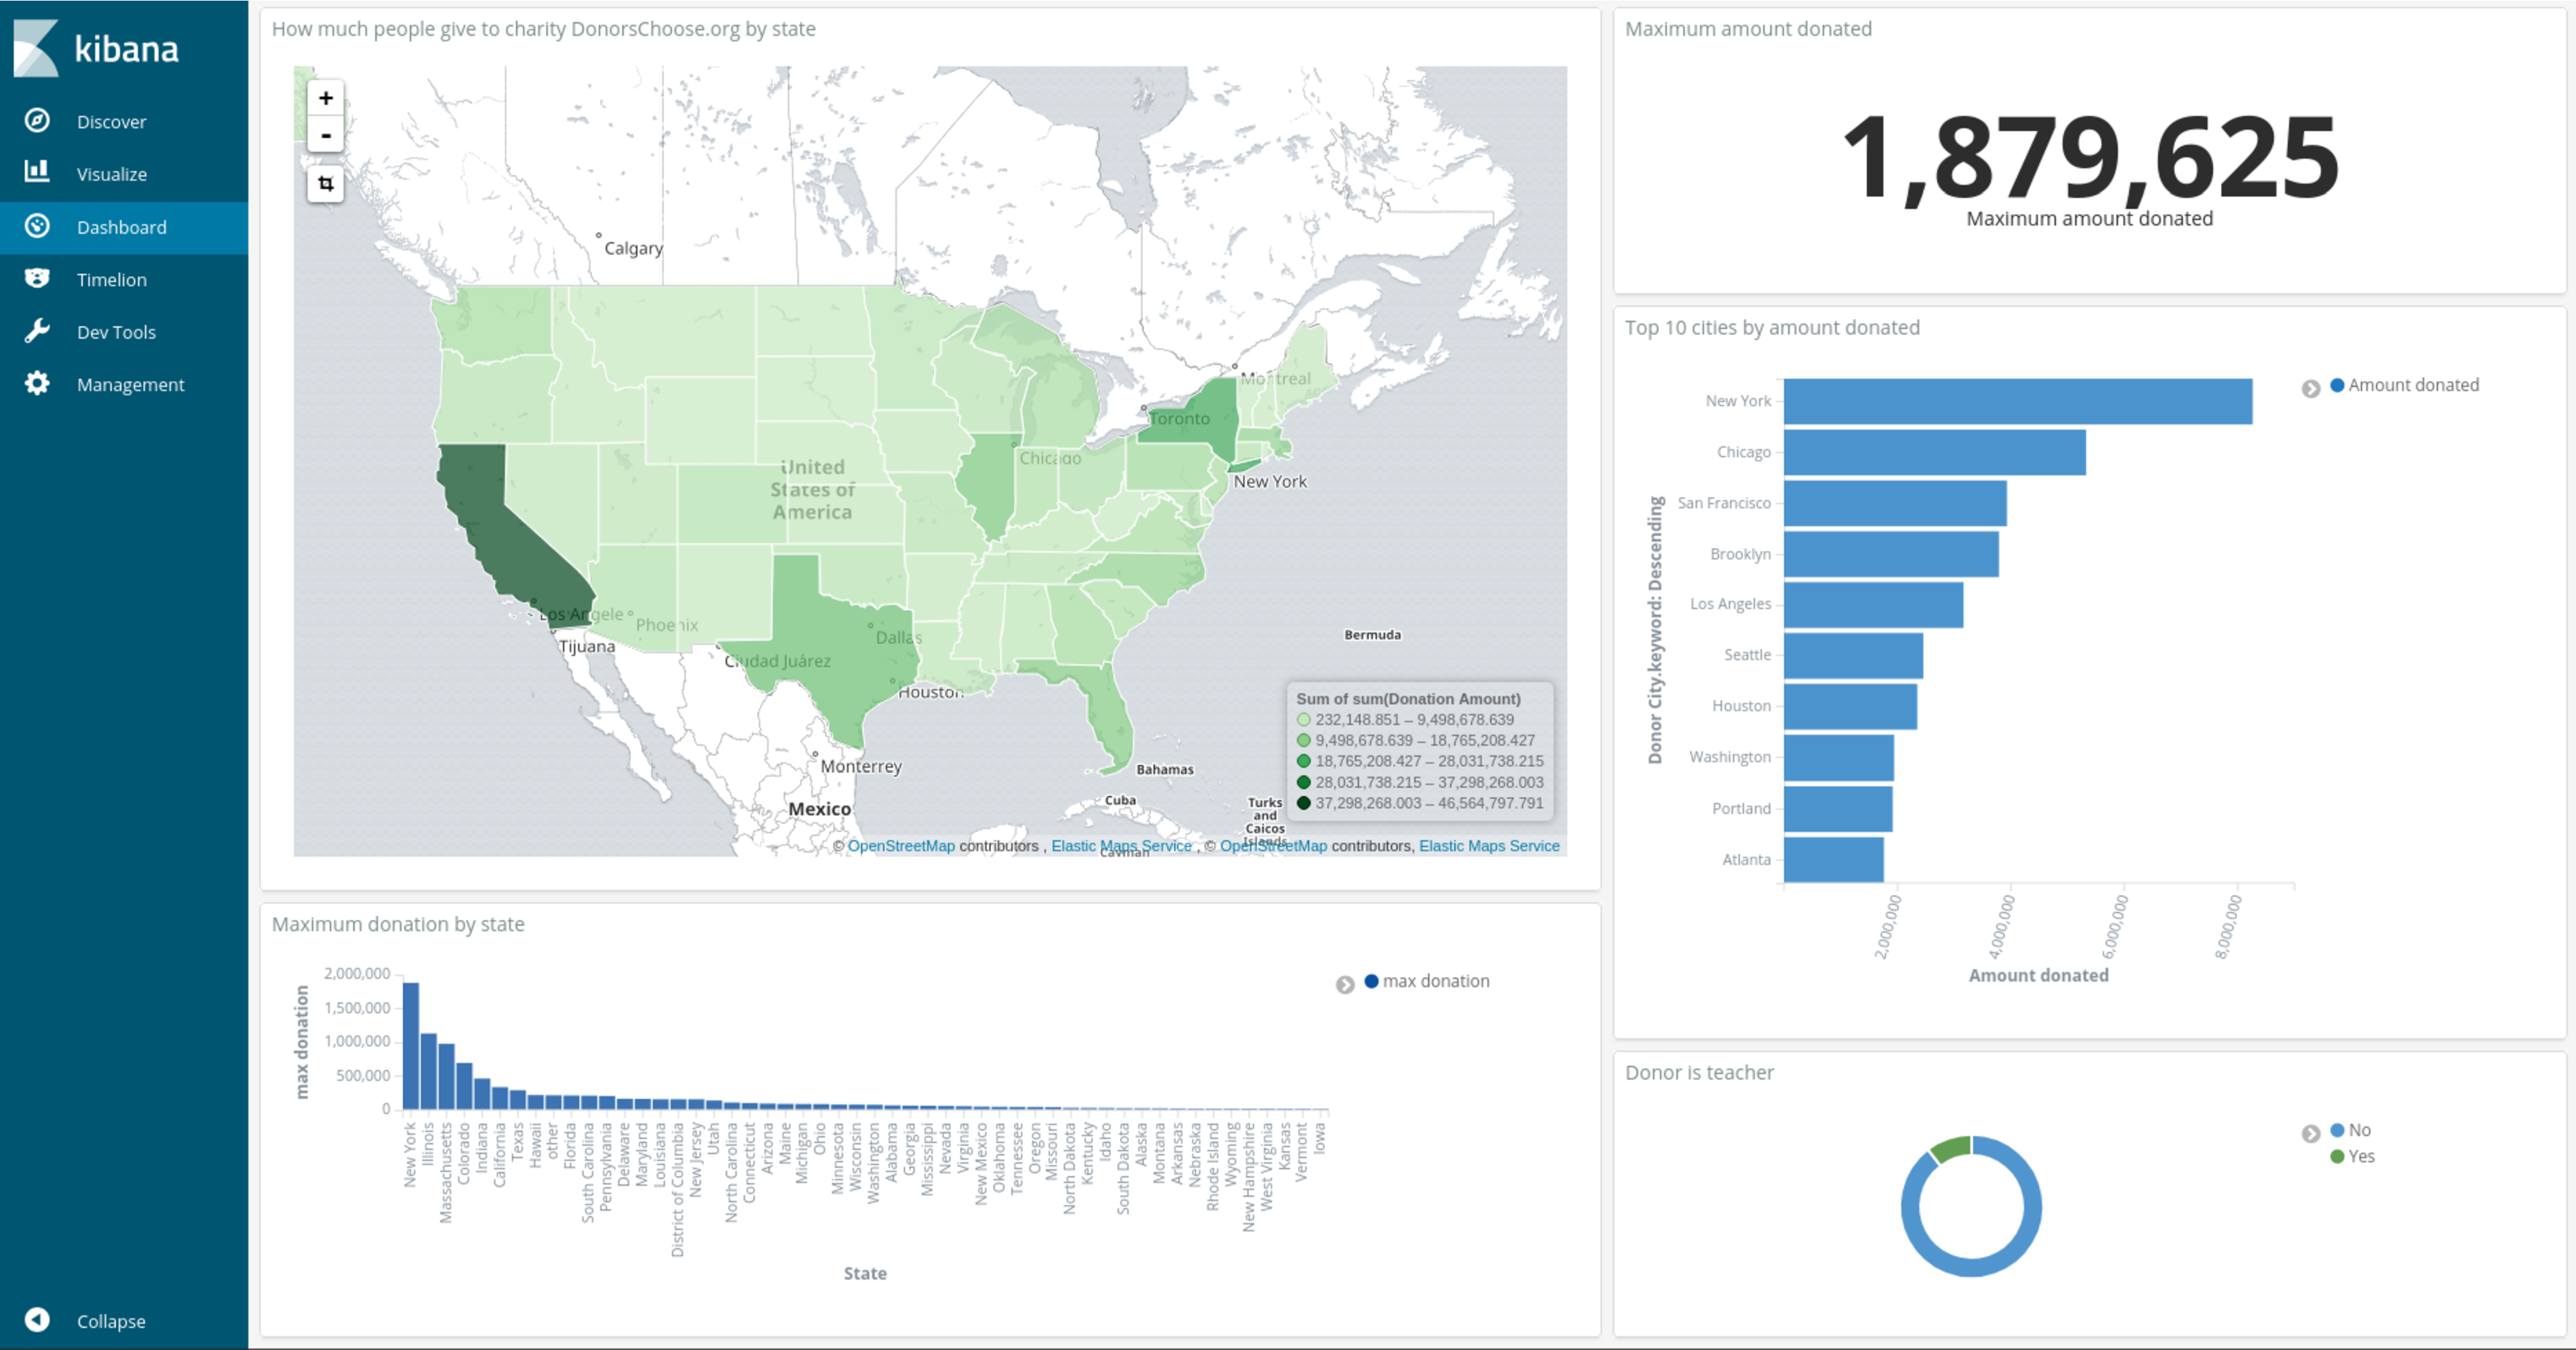
\includegraphics[width=16cm]{dashboard}
\end{center}

Mapa vlevo nahoře ukazuje součet darů všech lidí podle státu. Číslo vpravo nahoře ukazuje maximální součet darů od jednoho člověka. Pie chart vpravo dole ukazuje procentuální zastoupení učitelů mezi dárci a zbylé dva grafy porovnávají jednotlivá města podle součtu všech darů nebo maximálního daru. Obrázek v detailnější podobě najdete na adrese \url{https://www.dropbox.com/s/2p2a4e0fatuc5xu/dashboard.pdf?dl=0}.

\pagebreak
\subsection{Dotazy nad indexem}
Příkazy jsem zadával do Dev Tools v Kibaně\index{Kibana}.
\subsubsection{Filtrování}
Vypiš všechny dárce z města Hunstville.
\begin{lstlisting}
GET donationsbydonors/_search
{
  "query": {
    "match": {
      "Donor City": "Huntsville"
    }
  }
}
\end{lstlisting}

\subsubsection{Třídění}
Seřaď všechny dárce z města Hunstville podle velikosti součtu jejich darů.
\begin{lstlisting}
GET donationsbydonors/_search
{
  "sort":{
    "sum(Donation Amount)": { "order":"desc" }
    },
  "query": {
    "match": {
      "Donor City": "Huntsville"
    }
  }
}
\end{lstlisting}
\pagebreak
\subsubsection{Wildcard hledání}
Najdi všechny dárce kteří pochazejí z města končící na "ville".
\begin{lstlisting}
GET donationsbydonors/_search
{
  "query": {
    "wildcard": {
      "Donor City": "*ville"
    }
  }
}
\end{lstlisting}


\section{Závěr}
Během tvorby semestrální práce jsem si vyzkoušel práci s docker-compose a dalšími technologiemi pro práci s "big-data". Nejvíce časově náročné bylo nahrávání dat do nástrojů (Spark\index{Spark}, Elasticsearch\index{Elasticsearch}), ale většina následných operací byla rychlá. Z vizualizací dat jsme zjistili, že lidé ze státu California dávájí nejvíce na charitu ze všech států USA. Také jsme zjistili, že existuje zhruba desítka státu (např. Vermont), kde nejvyšší součet darovaných částek jednoho člověka se pohyboval v řádech několika stovek, což může indikovat, že v těchto státech není velké zastoupení bohatých nebo štědrých lidí. 


%%%%% REJSTRIK -->

\printindex

\newpage

%%%%% REJSTRIK <--


\end{document}
